\documentclass{article}


\usepackage[english]{babel}


\usepackage[letterpaper,top=2cm,bottom=2cm,left=3cm,right=3cm,marginparwidth=1.75cm]{geometry}


\usepackage{amsmath}
\usepackage{graphicx}
\usepackage[colorlinks=true, allcolors=blue]{hyperref}

\title{Video Game Sales Analysis}
\author{Chao Yuan}

\begin{document}
	\maketitle
	\section{Introduction}
	This project is based on the data set of video game sales from 1980 to 2017. In this report, I analyze game sales with many angles. For example, I show the relationship between global sales and year and I find out the top 10 game of different district. Through these analyses, we can summarize the sales of the game and provide some suggestions for the production of the game.
	
	\section{Data Analysis}
	
	\subsection{Global Sales By Year}
	\begin{figure}[htbp]
	\centering
	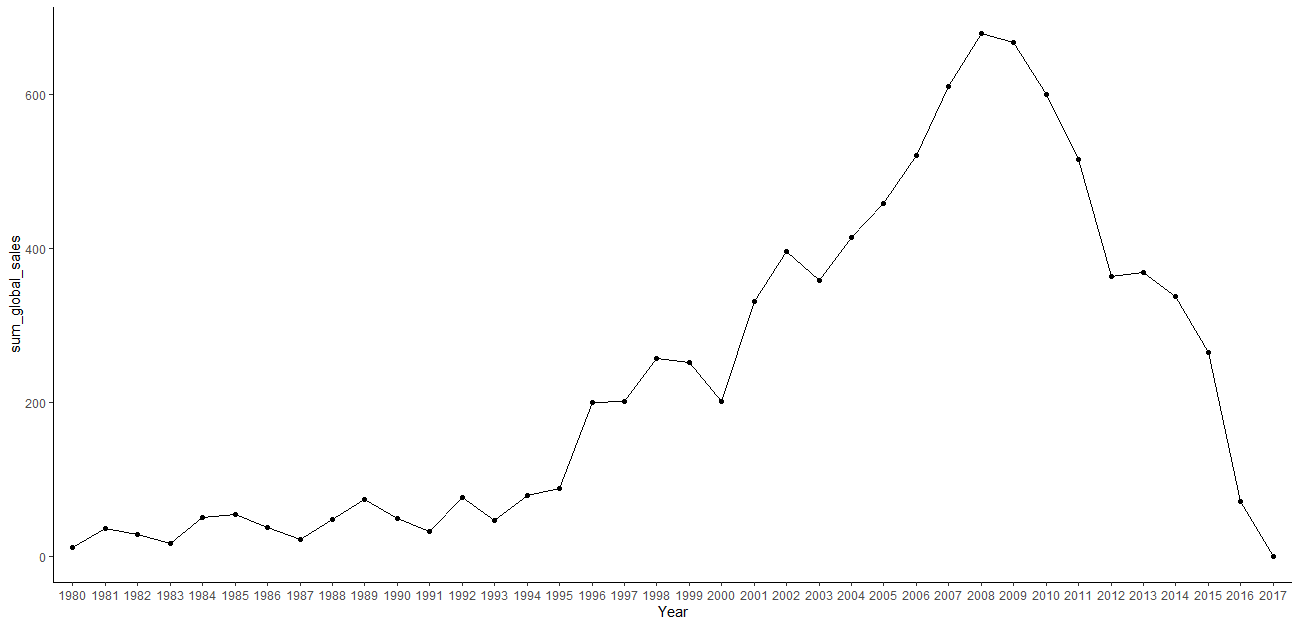
\includegraphics[scale = 0.4]{Year_sales.png}
	\end{figure}

	We can see from the figure that global game sales reached their peak in 2008. But what is puzzling is that after 2008, the total global game sales began to fall quickly. Even in 2016, its sales were about the same as in 1980. Firstly I thought it's a problem with the data set, but I find that some other people's results are similar to mine, so I don't know what happened. Perhaps global game sales are really declining, but the data set is also lacking in data.

	\newpage
	\subsection{Global Genre Sales }
	\begin{figure}[htbp]
	\centering
	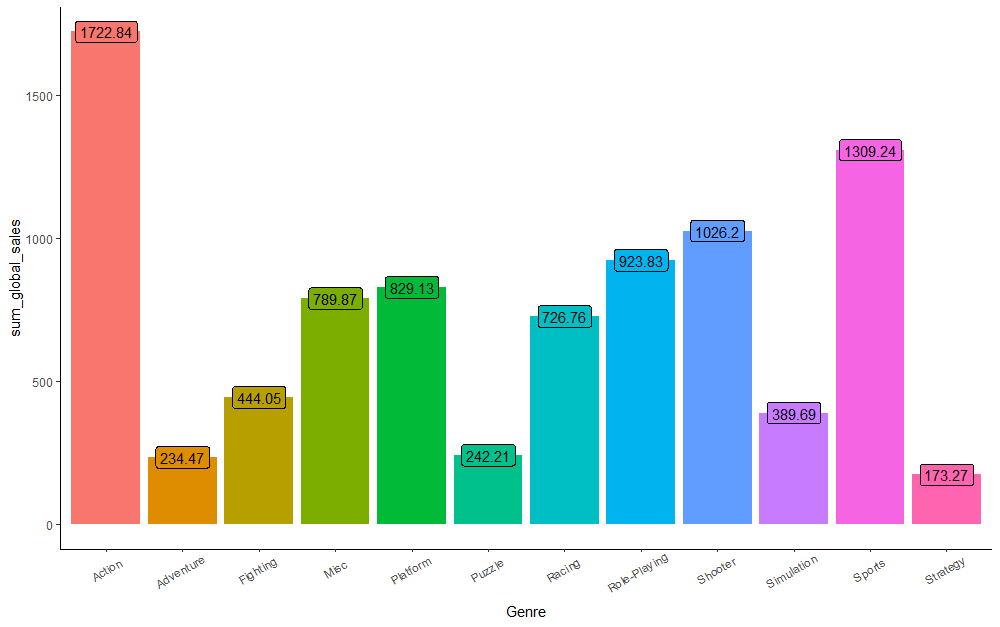
\includegraphics[scale = 0.4]{Genre_sales.png}
	\end{figure}
	In this figure, the three most popular game types are Action, Sport and Shooter. Role Playing games, Platform games and Racing games have similar sales. Misc means Miscellaneous Games and it makes no sense here. Additionally, Strategy games is least popular and it's only one of Action games.
	
	\subsection{TOP 10 Platform Sales}
		\begin{figure}[htbp]
		\centering
		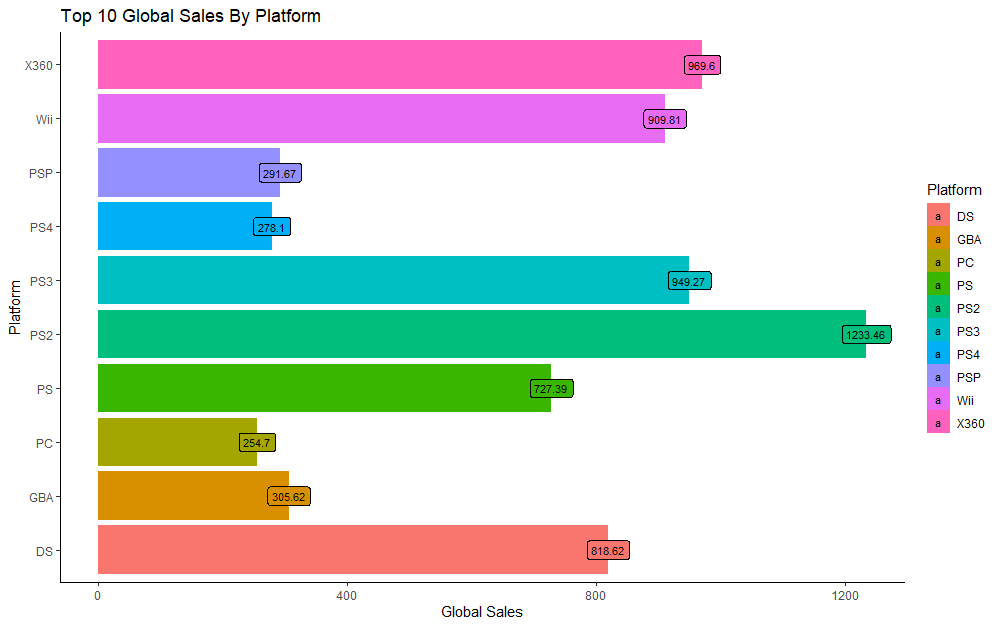
\includegraphics[scale = 0.5]{TOP10Platform.png}
		\end{figure}
	There is no doubt that Playstation, Xbox and Nintendo still dominate the game market. Playstation games accounts for the highest proportion and PS2 is most popular. Next is Nintendo games, which includes Wii and DS. The PC platform has the least proportion of the top 10 platforms although it's really convenient.
	
	\newpage
	\subsection{TOP 10 Publisher Sales}
	\begin{figure}[htbp]
		\centering
		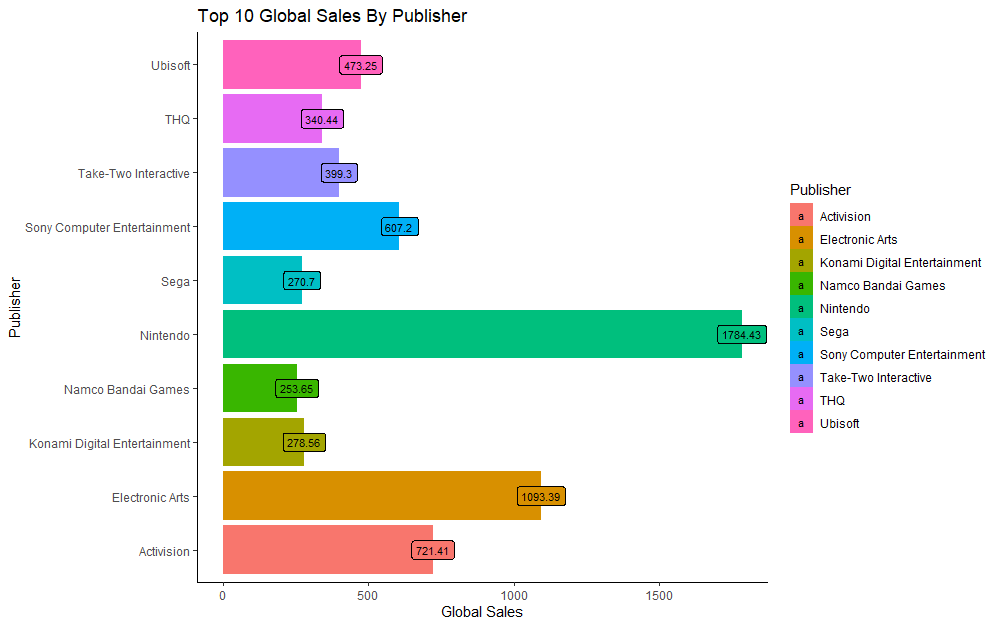
\includegraphics[scale = 0.5]{TOP10Publisher.png}
	\end{figure}
	Nintendo and EA account for almost half of global sales and Nintendo's performance is outstanding. Activision and Sony is close behind.
	
	\subsection{Game Sold Quantity By Genre}
	\begin{figure}[htbp]
		\centering
		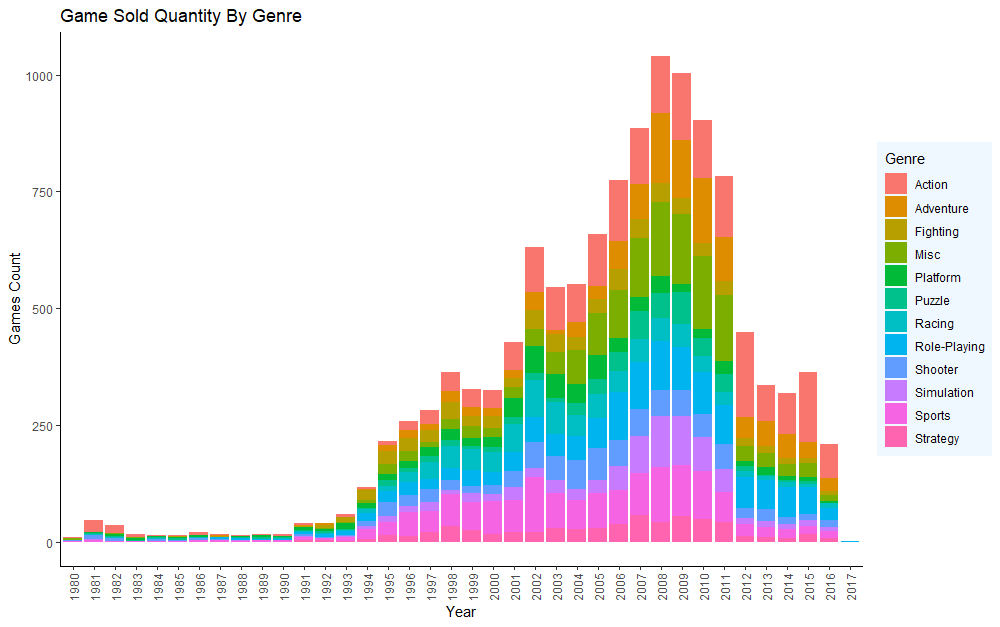
\includegraphics[scale = 0.5]{Genre_year.png}
	\end{figure}
	In this graph, we can compare the number of different genre of games sold in each year. A lot of games of various genres were sold around 2008.
	
	\newpage
	\subsection{TOP 10 Popular Games in each market}
	\begin{figure}[htbp]
		\centering
		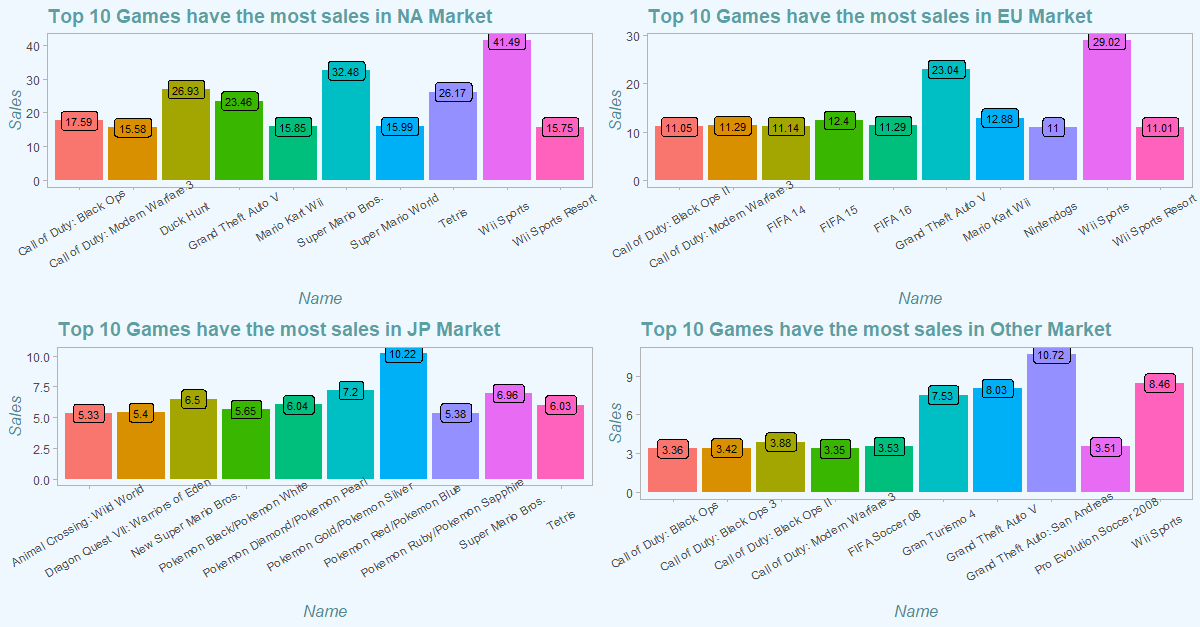
\includegraphics[scale = 0.5]{TOP10Game_each_market}
	\end{figure}
	We can easily conclude from this figure that people in different distinct love different genre of games. For example, Call of Duty is very popular in regions except Japan. People in North American and Japan don't like FIFA so much. The reasons for this phenomenon are complex because the culture of society is totally different. 
	
	

	
\end{document}